\chapter{Resultaten}
\label{sectie_psnr}
In dit hoofdstuk zullen we een kwantitatieve vergelijking tussen de verschillende algoritmes maken. Hierbij zullen we het begrip \emph{Peak Signal To Noise Ratio} introduceren, een veelgebruikte methode om de reconstructiequaliteit van een lossy compressie-algoritme te testen.

\begin{definitie}[Peak Signal To Noise Ratio (PSNR)]
  Gegeven een signaal $f: \Z^k \to \R^k$ en een reconstructie $\hat f$, is de $\operatorname{PSNR}$ gelijk aan
  \[
  \operatorname{PSNR}(f) := 20 \cdot \log_{10}( M ) - 10 \cdot \log_{10}(S),
  \]
  waarbij
  \[
  M := \max( \max_{\boldsymbol j \in \Z^k} (f[\boldsymbol j]), \max_{\boldsymbol j \in \Z^k} (\hat f[\boldsymbol j]))
  \]
  en
  \[
  S := \| f - \hat f \|_{\ell_2} = \sum_{\boldsymbol j \in \Z^k} (f[\boldsymbol j] - \hat f[\boldsymbol j])^2.
  \]
  Hoe hoger de PSNR is, hoe beter de reconstructie over het algemeen zal zijn.	
\end{definitie}

\subsection{Gebruikte testbeelden}
\label{testjes}
Met een beetje kwade wil kan altijd een beeld geconstrueerd worden dat met minder co\"effici\"enten is te schrijven
in de ene basis dan in de andere: voor een extreem voorbeeld zie figuur \ref{fig:sinus_fig}.
Omdat het object van studie een beeldcompressie-algoritme is, hebben wij ons gericht op een realistische vari\"eteit
beeldmateriaal waarvoor dit algoritme gebruikt zou kunnen worden. 
De afbeeldingen kunnen ruwweg verdeeld worden in een aantal categorie\"en:
\begin{description}
\item[Fotorealistische beelden] worden gekarakteriseerd door het ontbreken van scherpe randen hoewel
  er veel \emph{details} belangrijk zijn. Ook is het verloop in het beeld voornamelijk \emph{vloeiend}
  (zie figuren \ref{fig:lenna_start} - \ref{fig:lenna_eind}).
\item[Cartoony beelden] zijn over het algemeen minder complex (weinig belangrijke details en minder vloeiend) 
  en bestaat in het algemeen uit \emph{kleurvlakken} omgeven met \emph{scherpe randen}
  (zie figuren \ref{fig:shyguy_start} - \ref{fig:shyguy_eind}).
\item [Computer Graphics] spant een grotere categorie op die de \emph{scherpe randen} deelt met de Cartoony beelden
  maar ook veel \emph{vloeiende} verlopen heeft in plaats van kleurvlakken
  (zie figuren \ref{fig:gentoo_start} - \ref{fig:gentoo_eind}).
\item[Pixel Art] lijkt op de Cartoony beelden vanwege de \emph{scherpe randen} en \emph{kleurvlakken}
  maar heeft bijna altijd een enorme hoeveelheid \emph{details} aangezien het beeld pixel voor pixel vervaardigd is (zie figuur~\ref{fig:tensor_end}).
\end{description}

\begin{figure}[h]
  \centering
  \begin{subfigure}[b]{0.25\textwidth}
    \centering
    
\includegraphics[width=\textwidth]{plaatjes/sin_fourier.png}
  \end{subfigure}
  \begin{subfigure}[b]{0.25\textwidth}
    \centering
    
\includegraphics[width=\textwidth]{plaatjes/sin.png}
  \end{subfigure}
  \caption{Een periodiek signaal wordt perfect door de Fouriertransformatie gereconstrueerd door 1 \% van de data; de wavelettransformatie geeft hier een
echter een slechte reconstructie.}
  \label{fig:sinus_fig}
\end{figure}

\subsection{3D signalen}
Behalve de illustraties die op de volgende pagina's te zien zijn, hebben we ook een aantal bewegende beelden (3D-signalen) gecomprimeerd. Deze kunt u als lezer vinden door te navigeren naar de \url{gifjes/} submap en daar dubbel te klikken op \url{index.html}.

We hebben bij deze 3D-signalen niet Fourier vergeleken met Wavelets. Dit was het gevolg van praktische bezwaren 
(de Fouriertransformatie deed er simpelweg te lang over). 
Wel hebben we de Mallatdecompositie vergeleken met onze mengvorm: 
in het $(x,y)$-vlak gebruiken we de Mallatdecompositie in twee dimensies, 
met daar loodrecht op een Tensorproduct in de tijdsrichting.

\pagebreak
\newgeometry{left=2cm,right=2cm,top=1cm,bottom=1cm}
\begin{figure}
  \centering
  \begin{subfigure}[b]{0.24\textwidth}
    \centering
    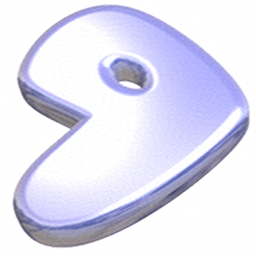
\includegraphics[width=\textwidth]{plaatjes/gentoo_fourier_0_15.png}
  \end{subfigure}
  \begin{subfigure}[b]{0.24\textwidth}
    \centering
    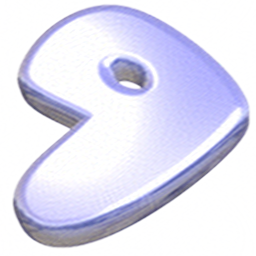
\includegraphics[width=\textwidth]{plaatjes/gentoo_fourier_0_1.png}
  \end{subfigure}
  \begin{subfigure}[b]{0.24\textwidth}
    \centering
    
\includegraphics[width=\textwidth]{plaatjes/gentoo_fourier_0_05.png}
  \end{subfigure}
  \begin{subfigure}[b]{0.24\textwidth}
    \centering
    
\includegraphics[width=\textwidth]{plaatjes/gentoo_fourier_0_01.png}
  \end{subfigure}
  \caption{Fourier op compressieniveaus 0.15, 0.10, 0.05, 0.01.}
  \label{fig:gentoo_start}
\end{figure}
\begin{figure}
  \centering
  \begin{subfigure}[b]{0.24\textwidth}
    \centering
    
\includegraphics[width=\textwidth]{plaatjes/gentoo_haar_0_15.png}
  \end{subfigure}
  \begin{subfigure}[b]{0.24\textwidth}
    \centering
    
\includegraphics[width=\textwidth]{plaatjes/gentoo_haar_0_1.png}
  \end{subfigure}
  \begin{subfigure}[b]{0.24\textwidth}
    \centering
    
\includegraphics[width=\textwidth]{plaatjes/gentoo_haar_0_05.png}
  \end{subfigure}
  \begin{subfigure}[b]{0.24\textwidth}
    \centering
    
\includegraphics[width=\textwidth]{plaatjes/gentoo_haar_0_01.png}
  \end{subfigure}
  \caption{Haar op compressieniveaus 0.15, 0.10, 0.05, 0.01.}
\end{figure}
\begin{figure}
  \centering
  \begin{subfigure}[b]{0.24\textwidth}
    \centering
    
\includegraphics[width=\textwidth]{plaatjes/gentoo_db2_0_15.png}
  \end{subfigure}
  \begin{subfigure}[b]{0.24\textwidth}
    \centering
    
\includegraphics[width=\textwidth]{plaatjes/gentoo_db2_0_1.png}
  \end{subfigure}
  \begin{subfigure}[b]{0.24\textwidth}
    \centering
    
\includegraphics[width=\textwidth]{plaatjes/gentoo_db2_0_05.png}
  \end{subfigure}
  \begin{subfigure}[b]{0.24\textwidth}
    \centering
    
\includegraphics[width=\textwidth]{plaatjes/gentoo_db2_0_01.png}
  \end{subfigure}
  \caption{Daubechies 2 op compressieniveaus 0.15, 0.10, 0.05, 0.01.}
  \label{fig:gentoo_eind}
\end{figure}
\begin{figure}
  \centering
  \begin{subfigure}[t]{0.48\textwidth}
    \centering
    \vspace{10pt}
    \begingroup

    \renewcommand*{\arraystretch}{1.5}
    $\begin{array}{c | c c c c}
      \text{Compr} & \text{Fourier} & \text{Haar} & \text{DB2} \\ \hline
      0.150 & -21.564987 & 1.508043 & -0.325757 \\
      0.125 & -22.220604 & -3.607729 & -4.753701 \\
      0.100 & -22.974077 & -7.518578 & -8.964313 \\
      0.075 & -23.893526 & -11.909545 & -13.080699 \\
      0.050 & -25.134504 & -17.028756 & -17.498265 \\
      0.040 & -25.786567 & -19.471026 & -19.515331 \\
      0.030 & -26.597406 & -21.936183 & -21.791275 \\
      0.020 & -27.693270 & -25.283096 & -24.377904 \\
      0.010 & -29.532364 & -28.763393 & -27.638580 \\ \hline
    \end{array}$
    \endgroup
  \end{subfigure}
  \begin{subfigure}[t]{0.48\textwidth}
    \centering
    \vspace{0pt}
    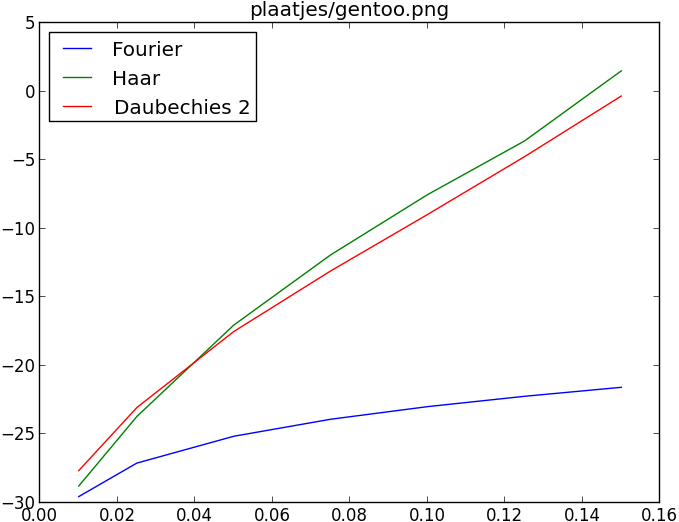
\includegraphics[height=\textwidth]{plaatjes/grafiek_gentoo_0_15-0_01.png}
  \end{subfigure}
\end{figure}
\restoregeometry
\pagebreak


\pagebreak
\newgeometry{left=2cm,right=2cm,top=1cm,bottom=1cm}
\begin{figure}
  \centering
  \begin{subfigure}[b]{0.24\textwidth}
    \centering
    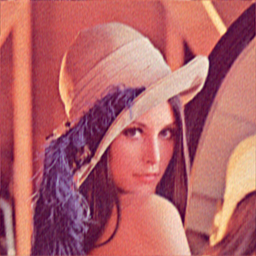
\includegraphics[width=\textwidth]{plaatjes/Lenna_fourier_0_1.png}
  \end{subfigure}
  \begin{subfigure}[b]{0.24\textwidth}
    \centering
    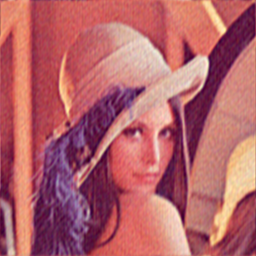
\includegraphics[width=\textwidth]{plaatjes/Lenna_fourier_0_05.png}
  \end{subfigure}
  \begin{subfigure}[b]{0.24\textwidth}
    \centering
    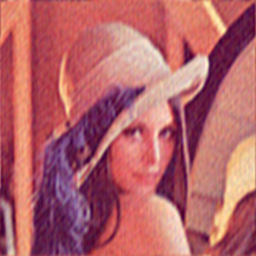
\includegraphics[width=\textwidth]{plaatjes/Lenna_fourier_0_03.png}
  \end{subfigure}
  \begin{subfigure}[b]{0.24\textwidth}
    \centering
    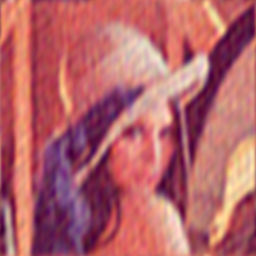
\includegraphics[width=\textwidth]{plaatjes/Lenna_fourier_0_01.png}
  \end{subfigure}
  \caption{Fourier op compressieniveaus 0.10, 0.05, 0.03, 0.01.}
  \label{fig:lenna_start}
\end{figure}
\begin{figure}
  \centering
  \begin{subfigure}[b]{0.24\textwidth}
    \centering
    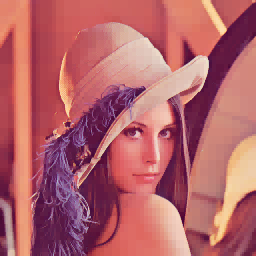
\includegraphics[width=\textwidth]{plaatjes/Lenna_haar_0_1.png}
  \end{subfigure}
  \begin{subfigure}[b]{0.24\textwidth}
    \centering
    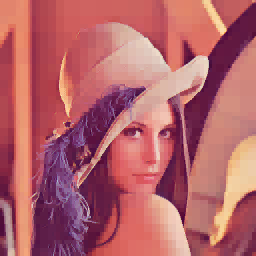
\includegraphics[width=\textwidth]{plaatjes/Lenna_haar_0_05.png}
  \end{subfigure}
  \begin{subfigure}[b]{0.24\textwidth}
    \centering
    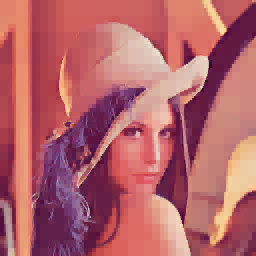
\includegraphics[width=\textwidth]{plaatjes/Lenna_haar_0_03.png}
  \end{subfigure}
  \begin{subfigure}[b]{0.24\textwidth}
    \centering
    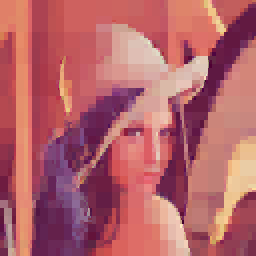
\includegraphics[width=\textwidth]{plaatjes/Lenna_haar_0_01.png}
  \end{subfigure}
  \caption{Haar op compressieniveaus 0.10, 0.05, 0.03, 0.01.}
\end{figure}
\begin{figure}
  \centering
  \begin{subfigure}[b]{0.24\textwidth}
    \centering
    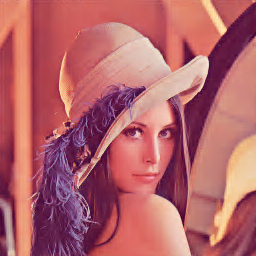
\includegraphics[width=\textwidth]{plaatjes/Lenna_db2_0_1.png}
  \end{subfigure}
  \begin{subfigure}[b]{0.24\textwidth}
    \centering
    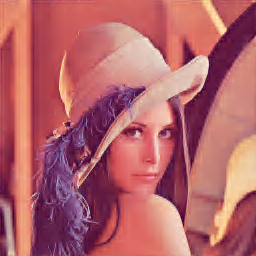
\includegraphics[width=\textwidth]{plaatjes/Lenna_db2_0_05.png}
  \end{subfigure}
  \begin{subfigure}[b]{0.24\textwidth}
    \centering
    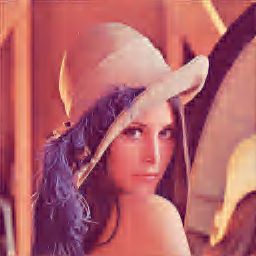
\includegraphics[width=\textwidth]{plaatjes/Lenna_db2_0_03.png}
  \end{subfigure}
  \begin{subfigure}[b]{0.24\textwidth}
    \centering
    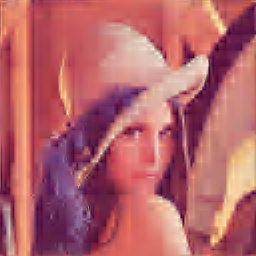
\includegraphics[width=\textwidth]{plaatjes/Lenna_db2_0_01.png}
  \end{subfigure}
  \caption{Daubechies 2 op compressieniveaus 0.10, 0.05, 0.05, 0.01.}
  \label{fig:lenna_eind}
\end{figure}
\begin{figure}
  \centering
  \begin{subfigure}[t]{0.48\textwidth}
    \centering
    \vspace{10pt}
    \begingroup

    \renewcommand*{\arraystretch}{1.5}
    $\begin{array}{c | c c c c}
      \text{Compr} & \text{Fourier} & \text{Haar} & \text{DB2} \\ \hline
      0.200 & -21.043701 & -16.443978 & -15.615197 \\
      0.100 & -23.867860 & -20.863769 & -20.134351 \\
      0.050 & -25.825943 & -24.400495 & -23.745103 \\
      0.040 & -26.362758 & -25.303459 & -24.684358 \\
      0.030 & -27.024421 & -26.407813 & -25.757180 \\
      0.020 & -27.928360 & -27.754692 & -27.139561 \\
      0.010 & -29.380617 & -29.651147 & -29.111878 \\ \hline
    \end{array}$
    \endgroup
  \end{subfigure}
  \begin{subfigure}[t]{0.48\textwidth}
    \centering
    \vspace{0pt}
    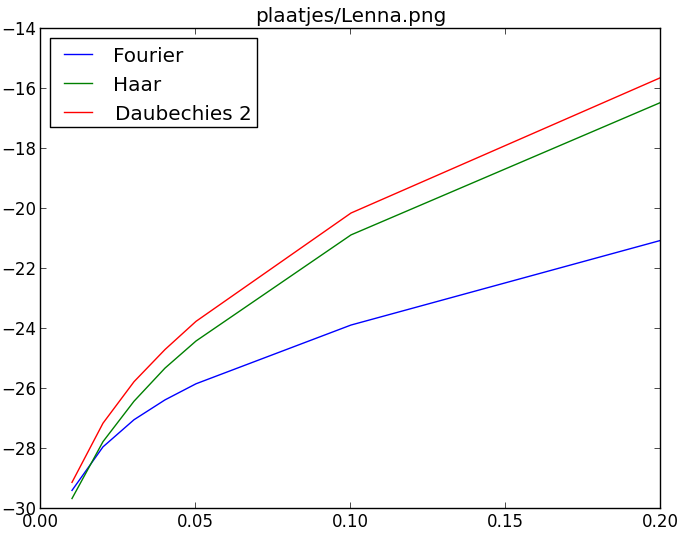
\includegraphics[height=\textwidth]{plaatjes/grafiek_Lenna_0_15-0_01.png}
  \end{subfigure}
\end{figure}
\restoregeometry
\pagebreak

\pagebreak
\newgeometry{left=2cm,right=2cm,top=1cm,bottom=1cm}
\begin{figure}
  \centering
  \begin{subfigure}[b]{0.24\textwidth}
    \centering
    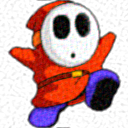
\includegraphics[width=\textwidth]{plaatjes/shyguy_fourier_0_1.png}
  \end{subfigure}
  \begin{subfigure}[b]{0.24\textwidth}
    \centering
    
\includegraphics[width=\textwidth]{plaatjes/shyguy_fourier_0_05.png}
  \end{subfigure}
  \begin{subfigure}[b]{0.24\textwidth}
    \centering
    
\includegraphics[width=\textwidth]{plaatjes/shyguy_fourier_0_03.png}
  \end{subfigure}
  \begin{subfigure}[b]{0.24\textwidth}
    \centering
    
\includegraphics[width=\textwidth]{plaatjes/shyguy_fourier_0_01.png}
  \end{subfigure}
  \caption{Fourier op compressieniveaus 0.10, 0.05, 0.03, 0.01.}
  \label{fig:shyguy_start}
\end{figure}
\begin{figure}
  \centering
  \begin{subfigure}[b]{0.24\textwidth}
    \centering
    
\includegraphics[width=\textwidth]{plaatjes/shyguy_haar_0_1.png}
  \end{subfigure}
  \begin{subfigure}[b]{0.24\textwidth}
    \centering
    
\includegraphics[width=\textwidth]{plaatjes/shyguy_haar_0_05.png}
  \end{subfigure}
  \begin{subfigure}[b]{0.24\textwidth}
    \centering
    
\includegraphics[width=\textwidth]{plaatjes/shyguy_haar_0_03.png}
  \end{subfigure}
  \begin{subfigure}[b]{0.24\textwidth}
    \centering
    
\includegraphics[width=\textwidth]{plaatjes/shyguy_haar_0_01.png}
  \end{subfigure}
  \caption{Haar op compressieniveaus 0.10, 0.05, 0.03, 0.01.}
\end{figure}
\begin{figure}
  \centering
  \begin{subfigure}[b]{0.24\textwidth}
    \centering
    
\includegraphics[width=\textwidth]{plaatjes/shyguy_db2_0_1.png}
  \end{subfigure}
  \begin{subfigure}[b]{0.24\textwidth}
    \centering
    
\includegraphics[width=\textwidth]{plaatjes/shyguy_db2_0_05.png}
  \end{subfigure}
  \begin{subfigure}[b]{0.24\textwidth}
    \centering
    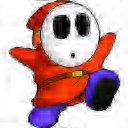
\includegraphics[width=\textwidth]{plaatjes/shyguy_db2_0_03.png}
  \end{subfigure}
  \begin{subfigure}[b]{0.24\textwidth}
    \centering
    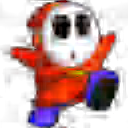
\includegraphics[width=\textwidth]{plaatjes/shyguy_db2_0_01.png}
  \end{subfigure}
  \caption{Daubechies 2 op compressieniveaus 0.10, 0.05, 0.05, 0.01.}
  \label{fig:shyguy_eind}
\end{figure}
\begin{figure}
  \centering
  \begin{subfigure}[t]{0.48\textwidth}
    \centering
    \vspace{10pt}
    \begingroup

    \renewcommand*{\arraystretch}{1.5}
    $\begin{array}{c | c c c c}
      \text{Compr} & \text{Fourier} & \text{Haar} & \text{DB2} \\ \hline
      0.125 & -25.709419 & 6.188436 & -12.939796 \\
      0.100 & -26.352690 & -2.252695 & -16.684428 \\
      0.075 & -27.084570 & -13.247047 & -20.121718 \\
      0.050 & -27.987835 & -22.194021 & -23.640705 \\
      0.040 & -28.455719 & -25.861219 & -25.259163 \\
      0.030 & -29.045916 & -26.633403 & -26.750137 \\
      0.020 & -29.857696 & -28.858775 & -28.445793 \\
      0.010 & -31.289113 & -31.320495 & -30.669577 \\ \hline
    \end{array}$
    \endgroup
  \end{subfigure}
  \begin{subfigure}[t]{0.48\textwidth}
    \centering
    \vspace{0pt}
    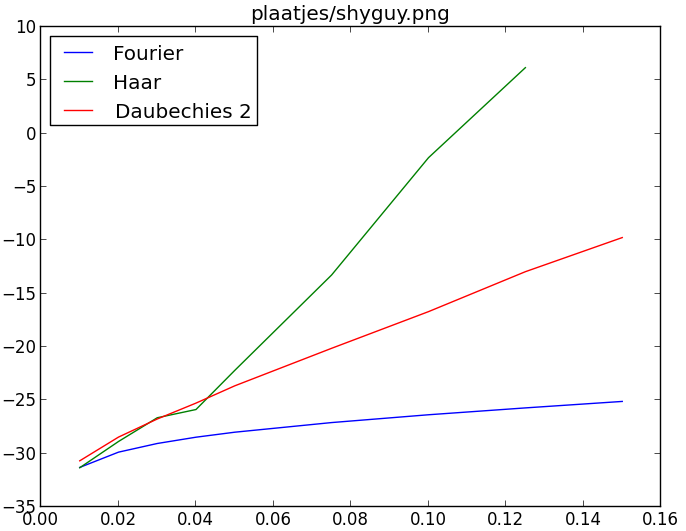
\includegraphics[height=\textwidth]{plaatjes/grafiek_shyguy_0_15-0_01.png}
  \end{subfigure}
\end{figure}
\pagebreak
\begin{figure}
	\centering
	\begin{subfigure}[t]{0.32\textwidth}
	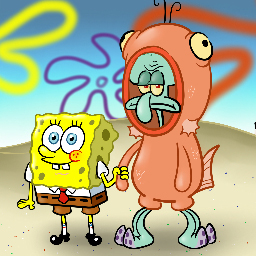
\includegraphics[width=\linewidth]{plaatjes/spongebob.jpg}
	\end{subfigure}
	\begin{subfigure}[t]{0.32\textwidth}
	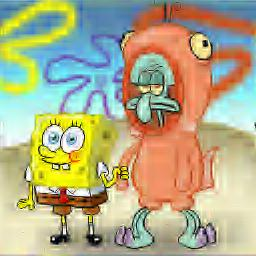
\includegraphics[width=\linewidth]{plaatjes/spongebob_db2_0_025.jpg}
	\end{subfigure}
	\begin{subfigure}[t]{0.32\textwidth}
	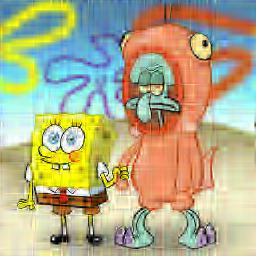
\includegraphics[width=\linewidth]{plaatjes/spongebob_db2_t_0_025.jpg}
	\end{subfigure}
	\caption{Links: \texttt{plaatjes/spongebob.jpg}. Midden: compressieniveau 0.025 met Daubechies 2. Rechts: compressie 0.025 met Daubechies-2 Tensor.}
	\label{fig:tensor_start}
\end{figure}
\begin{figure}
	\centering
	\begin{subfigure}[t]{0.48\textwidth}
	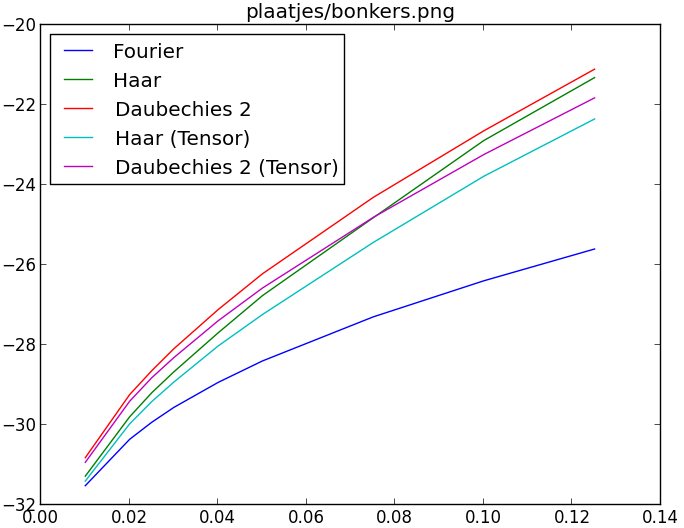
\includegraphics[width=\linewidth]{plaatjes/grafiek_bonkers.png}
	\caption{Grafiek horende bij de onderstaande afbeeldingen.}
	\end{subfigure}
	\begin{subfigure}[t]{0.48\textwidth}
	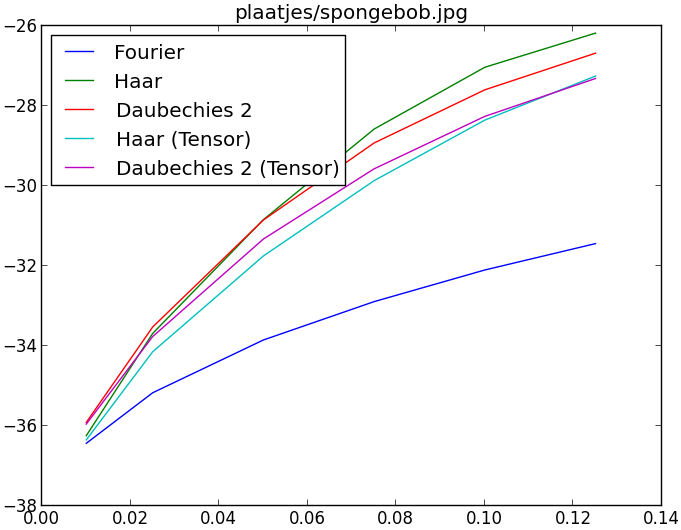
\includegraphics[width=\linewidth]{plaatjes/grafiek_spongebob_0_15-0_01.png}
	\caption{Grafiek horende bij de bovenstaande afbeeldingen.}
	\end{subfigure}
\end{figure}
\begin{figure}
	\centering
	\begin{subfigure}[t]{0.32\textwidth}
	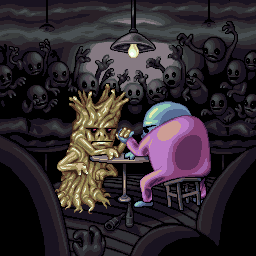
\includegraphics[width=\linewidth]{plaatjes/bonkers.png}
	\end{subfigure}
	\begin{subfigure}[t]{0.32\textwidth}
	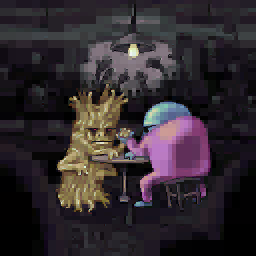
\includegraphics[width=\linewidth]{plaatjes/bonkers_haar_0_025.png}
	\end{subfigure}
	\begin{subfigure}[t]{0.32\textwidth}
	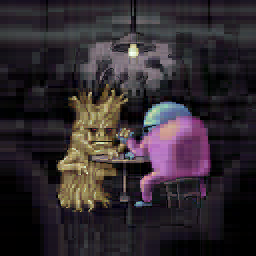
\includegraphics[width=\linewidth]{plaatjes/bonkers_haar_t_0_025.png}
	\end{subfigure}
	\caption{Links: \texttt{plaatjes/bonkers.png}. Midden: compressieniveau 0.025 met Haar. Rechts: compressie 0.025 met Haar Tensor.}
	\label{fig:tensor_end}
\end{figure}
\restoregeometry
\pagebreak
